\chapter{Background}

\section{Answer Set Programming (ASP)}

\subsection{Logic Program}

We will work on finite Logic Programs with rules of the form:
\begin{itemize}
\item $\leftarrow b_1, b_2, ..., b_m, \text{ not } c_1, \text{ not } c_2,...,\text{ not } c_n$ (also called \textit{constraint}).
\item $a \leftarrow b_1, b_2, ..., b_m, \text{ not } c_1, \text{ not } c_2,...,\text{ not } c_n$. This is a \textit{default} rule.
\item $l\{a_1, a_2, ..., a_p\}u \leftarrow b_1, b_2, ..., b_m, \text{ not } c_1, \text{ not } c_2,...,\text{ not } c_n$, where $l$ and $u$ are numbers such that $l \leq u$. Also, $l\{a_1, a_2, ..., a_p\}u$ is true in an Herbrand Interpretation $I$ iff $ l \leq |\{a_1, a_2, ..., a_p\}\cap I | \leq u$. This type of rule is also called \textit{choice rule}.
\end{itemize}
In all these rules, "$\text{ not }$" refers to the \textit{"negation as failure"}, and $a, a_1, a_2, ..., a_p, b_1, b_2,\\ ..., b_m, c_1, c_2, ...,  c_n$ are atoms. 

\smallskip

$a$ and $l\{a_1, a_2, ..., a_p\}u$ are called the \textit{head} of the rule, and $b_1, b_2, ..., b_m, \text{ not } c_1, \text{ not } c_2,\\..., \text{ not } c_n$ is the \textit{body} of the rule. If we call $r$ the following rule: $\alpha \leftarrow b_1, b_2, ..., b_m,\\ \text{ not } c_1, \text{ not } c_2,...,\text{ not } c_n$ where $\alpha$ is either an atom or an aggregate, then $body^+(r)=\{b_1, b_2,...,b_m \}$ and $body^-(r)=\{c_1, c_2,...,c_n \}$.

\smallskip

A \textit{literal} is an atom or the negation (by failure) of an atom.

\subsection{Stable Models (Answer Sets)}

Let $P$ be a logic program and $X$ be an Herbrand Interpretation of $P$. From $P$ and $X$, we can construct a new program $P^X$ called the \textit{reduct} of $P$ by applying these methods:
\begin{itemize}
\item For every rule $r\in P$, if $X\cap body^-(r)=\emptyset$, then we remove every negative literal in $r$.
\item Otherwise, if $X\cap body^-(r)\neq\emptyset$, then we delete the whole rule.
\item We replace every constraint $ :- body$ by $\perp :- body$. Here $\perp$ is an atom that does not appear in $P$. As a consequence, $\perp$ does not belong to any Answer Set.
\item For every rule $r$ with an aggregate in the head: $l\{a_1, a_2, ..., a_p\}u \leftarrow b_1, b_2, ..., b_m$ (we suppose that we have already removed the negative literals according to the first method)
\begin{itemize}
\item if $l \leq |\{a_1, a_2, ..., a_p\}\cap X | \leq u$, we replace $r$ by all the rules in the following set: $\{ a_i \leftarrow b_1, b_2, ..., b_m | a_i \in X\}$.
\item otherwise, we replace $r$ by $\perp \leftarrow b_1, b_2, ..., b_m$
\end{itemize}
\end{itemize}

Thus, the reduct $P^X$ is a \textit{definite} logic program (which means that it does not contain any negation as failure). Definite logic programs have a unique minimal Herbrand model, that is very easy to construct. We will write $M(P^X)$ the minimal Herbrand model of $P_X$.

\smallskip

We call \textit{stable model} of $P$ every Herbrand interpretation $X$ that satisfies the relation: $X=M(P^X)$. Moreover, as we do not use classical negation $\neg$, we will not make a distinction between \textit{answer sets} and stable models.

\smallskip

Stable models of $P$ have more properties than its models in general: they also are \textit{minimal} (for inclusion) and \textit{supported} (every atom in the stable model appears in a rule whose body evaluates to \textit{true}). 

\subsection{Tools}

For ASP problems, we will use some of the tools developed by the University of Potsdam: \texttt{gringo}, \texttt{clasp} and \texttt{clingo}. \texttt{gringo} transforms the logic program in input into an equivalent variable-free program (it is a \textit{grounder}). And \texttt{clasp} is a \textit{solver} capable of solving ground logic programs. Finally, \texttt{clingo} only combines grounding (with \texttt{gringo}) and solving (with \texttt{clasp}).

\smallskip

We used the version 4.3.0 of \texttt{clingo} since this the one that ILASP uses.
%TODO : reference manuel

\subsection{Optimization in clingo}

In \texttt{clingo}, it is possible to explain what kind of answer sets are optimal by using \textit{weak constraints}. A weak constraint has the following form:
\begin{center}
\texttt{:$\sim$ t$_1$, t$_2$, t$_3$,..., t$_n$.[w@p, id$_1$, id$_2$, ..., id$_m$]}
\end{center}
where \texttt{w} is called the \textit{weight}, and \texttt{p} is called the \textit{priority} of the weak constraint. We will also call \textit{ID} of the weak constraint the list \texttt{[\texttt{w}, \texttt{p}, id$_1$, id$_2$, ..., id$_m$]}. We say that a weak constraint is satisfied by an answer set $A$ if there is at least one atom among t$_1$, t$_2$, t$_3$,..., and t$_n$ that is not in $A$.

\smallskip

We call cost of an answer set $A$ for a given priority \texttt{p} (written $cost_{\texttt{p}}(A)$) the sum of the weights \texttt{w} of the different lists \texttt{[\texttt{w}, \texttt{p}, id$_1$, id$_2$, ..., id$_m$]} such that: there is at least a weak constraint whose ID is  \texttt{[\texttt{w}, \texttt{p}, id$_1$, id$_2$, ..., id$_m$]} that is not satisfied by $A$.

\bigskip

As a consequence:
\begin{itemize}
\item if we prefer the answer sets that satisfy a constraint \texttt{:- t$_1$, t$_2$, t$_3$,..., t$_n$.}, then we can use a weak constraint of the form \texttt{:$\sim$ t$_1$, t$_2$, t$_3$,..., t$_n$.[w@p, id$_1$, id$_2$, ..., id$_m$]} where the weight \texttt{w} is \textbf{positive}.
\item if we prefer the answer sets that satisfy all the atoms \texttt{t$_1$, t$_2$, t$_3$,...,} and \texttt{t$_n$} at the same time, then we can use a weak constraint of the form \texttt{:$\sim$ t$_1$, t$_2$, t$_3$,..., t$_n$.[w@p, id$_1$, id$_2$, ..., id$_m$]} where the weight \texttt{w} is \textbf{negative}.
\end{itemize}

\smallskip

For \texttt{clingo}, in a given ASP program $P$, an answer set $A_1$ \textbf{is preferred to} $A_2$ if and only if $cost_{\texttt{p}}(A_1)<cost_{\texttt{p}}(A_2)$ where \texttt{p} is the lowest priority for which $cost_{\texttt{p}}(A_1)\neq cost_{\texttt{p}}(A_2)$.

\begin{example}
We consider the following ASP program:\newline
\texttt{1\{go\_on\_holidays ; work\_at\_imperial\}1.\\
bad\_mark :- go\_on\_holidays.\\
good\_mark :- work\_at\_imperial.}

\smallskip

To this program we add the two following weak constraints:\newline
\texttt{:$\sim$ go\_on\_holidays.[-1@1] \% we enjoy holidays (priority 1)\\
:$\sim$ good\_mark.[-1@2] \% we like good marks (priority 2)}

\smallskip

This ASP program has two answer sets: $A_1 = \{ \texttt{go\_on\_holidays}, \texttt{bad\_mark}\}$ and $A_2 = \{ \texttt{work\_at\_imperial}, \texttt{good\_mark} \}$. 

\begin{itemize}
\item $A_1$ satisfies only the second weak constraint. So its scores are $cost_1(A_1)=-1$ and $cost_2(A_1)=0$.
\item $A_2$ satisfies only the first weak constraint. So its scores are $cost_1(A_2)=0$ and $cost_2(A_2)=-1$.
\end{itemize}

The highest priority is 2 and $cost_2(A_2)<cost_2(A_1)$. Thus, $A_2=\{ \texttt{work\_at\_imperial}, \texttt{good\_mark} \}$ is optimal.

\end{example}


%TODO : référence manuel ou référence à l'article évoqué dans manuel.

\section{Single-Player Games in ASP}

It is possible to formalize and solve Single-Player Games in ASP. To illustrate the predicates that can be used to describe these games, we will focus on a basic example: a simple graph game.

%TODO : référence 

\subsection{Rules of the game}

The rules of the graph game on figure \ref{fig:agent} are the following:
\begin{itemize}
\item The player starts in state $a$.
\item If the player is in state $a$ or in state $b$ then he can go to the left or to the right.
\item The player wins iff he goes to the state \textit{"victory"}.
\item The player cannot go back to state $a$ once he has reached the state \textit{"hole"}.
\end{itemize}

\begin{figure}[h]
\centering
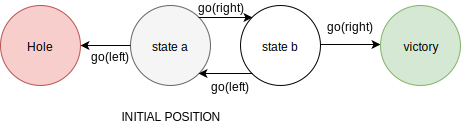
\includegraphics[width = 0.8\hsize]{figures/diagram1.png}
\caption{Simple graph game}
\label{fig:agent}
\end{figure}

\subsection{Describing the game in ASP}

\begin{itemize}

\item We start by defining the different players in the game by using the predicate \texttt{role}. Here, there is only one player so we include the fact: \texttt{role(player).}

\smallskip

\item Then, we define what are the initial states by using the predicate \texttt{holds} for the first time-step:\newline
\texttt{holds(hole, empty, 1).}\\
\texttt{holds(a, player, 1).} \% the player is in state $a$\\
\texttt{holds(b, empty, 1).}\\
\texttt{holds(victory, empty, 1).}

\item We also say what actions are legal at time $T$, depending on the state the player is:\newline
\texttt{legal(player,go(left),T) :- holds(a,player,T) ; holds(b,player, T)}\\
\texttt{legal(player,go(right),T) :- holds(a,player,T) ; holds(b,player,T)}

\item And we explain the situation at time $T+1$ depends on what holds at time $T$ and what the player does:\newline
\texttt{holds(hole,player,T+1) :- holds(a,player,T), does(player,go(left),T).}\\
\texttt{holds(b,player,T+1) :- holds(a,player,T), does(player,go(right),T).}\\
\texttt{...}

\item We can also define what is a \texttt{terminal} state, and we can evaluate each final state by using the predicate \texttt{goal}: \newline
\texttt{terminal(T) :- holds(victory, player, T).}\\
\texttt{terminal(T) :- holds(hole, player, T).}\\
\texttt{goal(player,100,T) :- holds(victory, player, T).}\\
\texttt{goal(player,  0,T) :- holds(hole, player, T).}
\end{itemize}

All these rules are \textbf{describing} the game in ASP.

\bigskip

We will respect the following Game Description Language (GDL) restriction: as long as we \textbf{describe} the game in ASP (and do not want to \textbf{simulate} a game play), the predicate \texttt{does} only appears in rule bodies, and does not appear in the definition of \texttt{terminal}, \texttt{goal} or \texttt{legal}.

\subsection{Finding a solution to the game/Simulating a gameplay}

We have just defined a few predicates to translate the rules of the game in ASP. Now we want to \textbf{simulate} a game play and find winning sequences of moves.
\begin{itemize}
\item First of all, the player can do only one move at every time step (as long as the game is not finished).\newline
\texttt{1\{does(player,go(left),T);does(player,go(right),T)\}1 :- not terminated(T).}\\
Where \texttt{terminated(T)} is true if and only if there is a T1 such that $T1<T$ and \texttt{terminal(T1)} is true:\newline
\texttt{terminated(T) :- terminal(T).}  \\
\texttt{terminated(T+1) :- terminated(T).}

\item Also, every move that is played must be legal:\newline
\texttt{:- does(player, M, T), not legal(player, M, T).}

\item We want the game to terminate at some point:\newline
\texttt{:- 0\{terminated(T) : time\_domain(T)\}0.}\\
\texttt{time\_domain(1..10). \% We allow at most 10 moves} 

\item Finally, we would like to find a sequence of moves in order to win the game:\newline
\texttt{:- terminal(T), not goal(player, 100, T)}

\end{itemize}

\section{Inductive Logic Programming}

In this part, $B$ is the logic program that represents the \textit{Background Knowledge}, $S_M$ is the set of possible hypotheses, $E^+$ is the set of positive examples (all the elements that have been observed) and $E^-$ is the set of negative examples (all the elements that can't appear in any result). Our task is to find an hypothesis $H\in S_M$ such that $B\cup H$ \textit{explains} $E^+$ and $E^-$. There are different ways of defining the word "explains" used in the last sentence. We will have a look at three of them.

%TODO S_M ???

\subsection{Brave Inductive Logic Programming}

\subsubsection{Brave Induction}

\begin{definition}

A brave inductive task is a tuple $T_b=<B, S_M, E^+, E^->$ where $E^+$ and $E^-$ are sets of atoms occurring in $B$. 

\smallskip

A hypothesis $H$ is solution of $T_b$ iff there is an answer set $A$ of $B\cup H$ verifying $E^+\subseteq A$ and $E^-\cap A = \emptyset$

\smallskip

We call $ILP_b(B,E^+,E^-)$ the set of hypotheses that are solutions of $T_b$. 

\end{definition}

\subsubsection{ASPAL encoding}

By using ASPAL, we can find the optimal solutions to a brave inductive task. We
illustrate how to use the ASPAL encoding with clingo in the following example.\bigskip

First of all, we consider the background knowledge B:\newline
\texttt{person(Nicolas). person(Pierre).\\
play\_video\_games(Nicolas). play\_video\_games(Pierre). works(Nicolas).}\\

And we take: $E^+=\{\texttt{good\_marks(Nicolas)}\}$ and $E^-=\{\texttt{good\_marks(Pierre)}\}$

\begin{itemize}
\item We are studying the hypotheses that are following this mode: \texttt{modeh(good\_marks(+X))}, \texttt{modeb(1,works(+X))} and \texttt{modeb(1,play\_video\_games(+X))}. So we write all the possible hypotheses, and we add the predicate rule/1 that takes as an argument the id of the hypothesis.\newline
\texttt{good marks(P) :- rule(1).\\
good\_marks(P) :- works(P), rule(2).\\
good\_marks(P) :- play\_video\_games(+P), rule(3).\\
good\_marks(P) :- works(P), play\_video\_games(+P), rule(4).}

\item We will select some rules between those above:\newline
\texttt{\{rule(1..4).\}}

\item And we want to respect the examples:\newline
\texttt{goal :- good\_marks(Nicolas), not good\_marks(Pierre).\\
:- not goal.}

\item Finally, we want to find the optimal (the shortest) hypothesis:\newline
\texttt{\#minimize[rule(1)=1,rule(2)=2,rule(3)=2,rule(4)=3].}

\end{itemize}




%TODO défauts d'ASPAL

\subsection{Cautious Inductive Logic Programming}

\begin{definition}

A cautious inductive task is a tuple $T_c=<B, E^+, E^->$ where $E^+$ and $E^-$ are sets of atoms occurring in $B$.

\smallskip

A hypothesis $H$ is solution of $T_c$ iff 
\begin{itemize}
\item $B\cup H$ has at least one answer set
\item every answer set of $B\cup H$ verifies $E^+\subseteq A$ and $E^-\cap A = \emptyset$
\end{itemize}

\smallskip

We call $ILP_c(B,E^+,E^-)$ the set of hypotheses that are solutions of $T_c$. 

\end{definition}

%TODO pas possible avec clingo

\subsection{Inductive Learning From Answer Sets Programming}

We present here a new type of inductive task which is more general than the cautious and the brave inductive tasks.

\subsubsection{Partial Interpretations}

We call \textit{partial interpretation} a tuple $<e^+,e^->$ where $e^+=\{e^+_1,e^+_2,...,e^+_m\}$ and $e^-=\{e^-_1,e^-_2,...,e^-_n\}$ are two sets of atoms.

\smallskip

We say that an interpretation $I$ of $B$ extends a partial interpretation $<e^+,e^->$ iff $e^+ \subseteq I$ and $e^- \cap I = \emptyset$.

\subsubsection{Learning from Answer Sets Induction}

\begin{definition}

A \textit{Learning from Answer Sets task} is a tuple $T_{LAS}=<B, S_M, E^+, E^->$ where $S_M$ is the hypothesis space; and $E^+$ and $E^-$ are sets of partial interpretations. 

\smallskip

An hypothesis $H$ is solution of $T_{LAS}$ iff 
\begin{itemize}
\item $H\subseteq S_M$
\item For all  $<e^+,e^->\in E^+$, there is an answer set of $B\cup H$ that extends $<e^+,e^->$
\item For all  $<e^+,e^->\in E^-$, there are no answer sets of $B\cup H$ that extend $<e^+,e^->$
\end{itemize}

We call $ILP_{LAS}(B,S_M,E^+,E^-)$ the set of hypotheses that are solutions of $T_{LAS}$. 
\end{definition}

\begin{example}

For example, we consider the following background knowledge $B$:

\texttt{student(Nicolas). \% Nicolas works and sleeps\\
works(Nicolas).\\
sleeps(Nicolas).\\
\\
student(Pierre). \% Pierre only works\\
works(Pierre). \\
\\
student(Jean). \% Jean only sleeps\\
sleeps(Jean). \\
\\
1\{good\_mark(P); bad\_mark(P)\}1 :- student(P). \% a student can have a either \\
											\% a good or a bad mark}
											
with the following hypothesis space $S_M$: \\
$\{$ \texttt{good\_mark(P) :- student(P).\\
good\_mark(P) :- student(P), sleeps(P).\\
good\_mark(P) :- student(P), works(P).\\
good\_mark(P) :- student(P), works(P), sleeps(P).} $\}$\\
and the following positive and negative examples: \\$E^+=\{<\{\texttt{bad\_mark(pierre),bad\_mark(jean)}\},\emptyset>\}$ \\and $E^-=\{<\{\texttt{bad\_mark(nicolas)}\},\emptyset>\}$.

\bigskip

First, $\emptyset$ is not a valid solution, as $\emptyset\cup H$ has an answer set which contains $\texttt{bad\_mark(nicolas)}$ and which consequently extends the negative example. With the first hypothesis, there is an answer set that satisfies the positive example, but there is also an answer set that extends the negative example. With the next two hypotheses, there are no answer sets that satisfy the negative example, but the positive example is never satisfied. With the last hypothesis, Nicolas is sure to have a good grade (the negative example is not extended by any answer set), and there is an answer set that contains both \texttt{bad\_mark(pierre)} and \texttt{bad\_mark(jean)}.

\bigskip

Thus $ILP_{LAS}(B,S_M,E^+,E^-)=\{\texttt{good\_mark(P) :- student(P), works(P), sleeps(P).}\}$

\end{example}

\begin{remark}

Every brave or cautious inductive task is a Learning from Answer Sets task. But the inverse is not true.

%TODO : reference paper
%TODO : proof ? in appendix ?

\end{remark}

\begin{proof}

\proofpart{1}{A brave inductive task is a Learning from Answer Sets task}
We consider the following brave inductive task: $T_b=<B,S_M,$ $\{e^+_1, e^+_2,...,e^+_m\},$ $\{e^-_1,...,e^-_n\}>$, and the following Learning from Answer Sets task: $T_{LAS}=<B,S_M,$ $\{p^+\},$ $\emptyset>$ where $p^+=<\{e^+_1, e^+_2,...,e^+_m\},$ $\{e^-_1,...,e^-_n\}>$.

\smallskip

\begin{tabular}{cc}
An hypothesis $H$ is solution of $T_{LAS}$ iff & \makecell[tl]{ $H\subseteq S_M$ and there is an answer set $A$ of\\ $B\cup H$ such that $A$ extends $p^+$}\\\\
\makecell[r]{iff} & \makecell[tl]{ $H\subseteq S_M$ and there is an answer set $A$ of\\ $B\cup H$ such that $A$ extends $p^+$}\\\\
\makecell[r]{iff} & \makecell[tl]{ $H\subseteq S_M$ and there is an answer set $A$ of\\ $B\cup H$ that contains all the $e^+_i$ and that \\does not contain any of the  $e^-_i$}\\\\
\makecell[r]{iff} & \makecell[tl]{ $H$ is solution of $T_b$}
\end{tabular}

\bigskip

So, the two tasks $T_b$ and $T_{LAS}$ are equivalent. Thus, we can construct a Learning from Answer Sets task from every brave inductive task.
 
\proofpart{2}{A cautious inductive task is a Learning from Answer Sets task}
 
We consider the following cautious inductive task: $T_c=<B,S_M,$ $\{e^+_1, e^+_2,...,e^+_m\},$ $\{e^-_1,...,e^-_n\}>$, and the following Learning from Answer Sets task: $T_{LAS}=<B,S_M,\emptyset,$ $\{p^-_1,...,p^-_m, q^-_1,...,q^-_n\}>$ where where for all $i$, $p^-_i=<\emptyset,\{e^+_i\}>$ and $q^-_i=<\{e^-_i\},\emptyset>$.

\smallskip

We can notice that an answer set $A$ extends $p^-_i$ iff $e^+_i\not \in A$. In addition, $A$ extends $q^-_i$ iff $e^-_i \in A$.

\smallskip

\begin{tabular}{cc}
\makecell{An hypothesis $H$ is solution of $T_{LAS}$ iff} & \makecell[lt]{ $H\subseteq S_M$ and for every answer set $A$ of\\ $B\cup H$, $A$ does not extend $p^-_i$ and $q^-_i$\\ (for all $i$)}\\\\
\makecell[r]{iff} & \makecell[tl]{$H\subseteq S_M$ and for every answer set $A$ of\\ $B\cup H$, $A$ contains $e^+_i$ and \\does not contain $e^-_i$ (for all $i$)}\\\\
\makecell[r]{iff} & \makecell[tl]{ $H$ is solution of $T_c$}\\
\end{tabular}

\bigskip

So, the two tasks $T_c$ and $T_{LAS}$ are equivalent. Thus, we can construct a Learning from Answer Sets task from every cautious inductive task.

\end{proof}

\subsubsection{Learning from Ordered Answer Sets}

The definition of Learning from Answer Sets task can be extended to take into account the ordering relations between the different answer sets of the ASP program. We will first define what is an ordering example, and how it can be used to represent the ordering relations \citep{law2015weak}.

\begin{definition}

We will call \textit{ordering example} every pair $<e_1,e_2>$ of partial interpretations. These are two ways for an ASP program to cover an ordering example:
\begin{itemize}
\item An ordering example is \textit{bravely covered} by an ASP program $P$ iff \textbf{there are} two answer sets $A_1$ and $A_2$ such that $A_1$ extends $e_1$, $A_2$ extends $e_2$ and $A_1$ is preferred to $A_2$.
\item An ordering example is \textit{cautiously covered} by an ASP program $P$ iff \textbf{for every} answer sets $A_1$ and $A_2$ such that $A_1$ extends $e_1$ and $A_2$ extends $e_2$ we have : $A_1$ is preferred to $A_2$.
\end{itemize}
\end{definition}

Now we can give the definition for a Learning from Ordered Answer Sets task \citep{law2015weak}:

\begin{definition}
A \textit{Learning from Ordered Answer Sets task} is a tuple $T_{LOAS}=<B, S_M, E^+, E^-,O^{brave}, O^{cautious}>$ (where $<B,S_M, E^+, E^->$ is a Learning from Answer Sets task, and $O^{brave}$ and $O^{cautious}$ are sets of ordering examples) such that: every partial interpretation that appears in $O^{brave}$ and $O^{cautious}$ is in $E^+$.

\smallskip

A hypothesis $H$ is solution of $T_{LOAS}$ iff 
\begin{itemize}
\item $H$ is a solution of $T_{LAS}=<B, S_M, E^+, E^->$.
\item Every ordering example in $O^{brave}$ is bravely covered by $B\cup H$
\item Every ordering example in $O^{cautious}$ is cautiously covered by $B\cup H$
\end{itemize}

We call $ILP_{LOAS}(B,S_M,E^+,E^-,O^{brave},O^{cautious})$ the set of hypotheses that are solutions of $T_{LOAS}$.
\end{definition}

\begin{example}
The week preceding an exam, a student has to decide if he will work or not. And at the end, he will get a mark that is good or not: $B=\{\texttt{0\{works\}1. 
0\{good\_mark\}1.}\}$

\bigskip

We define three positive examples: $e_1 = <\{\texttt{good\_mark}\},\{\texttt{works}\}>$, $e_2 = <\{\texttt{good\_mark},\texttt{ works}\},\emptyset>$ and $e_3 = <\emptyset,\{\texttt{good\_mark}\}>$. $E^+=\{e_1, e_2, e_3\}$. Besides, we take $E^-=\emptyset$.

\bigskip

Now we define the student's preferences:
\begin{itemize}
\item For him, having a good mark without working is better than having a good mark by working hard: $O^{brave}=\{<e_1,e_2>\}$
\item The student always prefers having a good grade without working than having a bad grade: $O^{cautious}=\{<e_1,e_3>\}$
\end{itemize}

Finally, we define the hypothesis space $S_M$:\\
$\{$ \texttt{:$\sim$ not works.[-1@1]\\
:$\sim$ good\_mark.[-1@1]\\
:$\sim$ not works, good\_mark.[-1@1]} $\}$\\

\bigskip

With the first hypothesis only, the answer set $A_1=\{$\texttt{good\_mark}$\}$ extends $e_1$, and $A_3=\emptyset$ is an other answer set that extends $e_3$. In this case, $cost_1(A_1)=cost_1(A_3)=-1$, so the ordering example in $O^{cautious}$ is not cautiously covered.

\bigskip

With the second hypothesis only, the only answer set that extends $e_1$ is $A_1=\{$\texttt{good\_mark}$\}$, and $A_2=\{$\texttt{good\_mark}$,$ \texttt{works}$\}$ is the only answer set that extends $e_2$. In this case, $cost_1(A_1)=cost_1(A_2)=-1$, so the ordering example in $O^{brave}$ is not bravely covered.

\bigskip

The last hypothesis respects all the brave and cautious orderings. Indeed $cost_1(A_1)=-1$ whereas for every answer set $A$ different form $A_1$, we have: $cost_1(A)=0$. But this is not the only hypothesis in $ILP_{LOAS}(B,S_M,E^+,E^-)$, as $H=\{$\texttt{:$\sim$ not works.[-1@1], :$\sim$ good\_mark.[-1@1]}$\}$ is also a solution (of length 2).

\bigskip

To conclude \texttt{:$\sim$ not works, good\_mark.[-1@1]} is \textbf{an} optimal (shortest) hypothesis of  $ILP_{LOAS}(B,S_M,E^+,E^-)$

\end{example}

\subsubsection{Learning from Context Dependant Answer Sets}
%TODO : talk about ILASP --2i

The task defined above can be generalized by adding a \textit{context} to every partial interpretation \citep{law2016context}. A \textit{context} is an ASP program that does not contain any weak constraint or any other statement used to classify answer sets. Instead of containing partial interpretations, $E^+$ and $E^-$ contain tuples $<<e^+,e^->,C>$ where $<e^+,e^->$ is a partial interpretation, and $C$ is the \textit{context} of this partial interpretation. 

\bigskip

As the definitions of positive and negative examples have been generalized by adding contexts, we need to extend the definition of an ordering example \citep{law2016context}.

\begin{definition}

We will call \textit{Context-Dependant Ordering Example} every pair $<<e_1,C_1>,<e_2,C_2>>$ where $e_1$ and $e_2$ are partial interpretations, and $C_1$ and $C_2$ are respectively the contexts of $e_1$ and $e_2$. These are two ways for an ASP program to cover an ordering example:
\begin{itemize}
\item An ordering example is \textit{bravely covered} by an ASP program $P$ iff \textbf{there is} an answer set $A_1$ of $P\cup C_1$ and \textbf{there is} an answer set $A_2$ of $P\cup C_2$ such that $A_1$ extends $e_1$, $A_2$ extends $e_2$ and $A_1$ is preferred to $A_2$.
\item An ordering example is \textit{cautiously covered} by an ASP program $P$ iff \textbf{for every} answer set $A_1$ of $P\cup C_1$ and \textbf{every} answer set $A_2$ of $P\cup C_2$ such that $A_1$ extends $e_1$ and $A_2$ extends $e_2$, we have: $A_1$ is preferred to $A_2$.
\end{itemize}

\end{definition}
%TODO : coverage ????
Now that we have a definition for Context-Dependant Ordering Examples, for brave coverage and for cautious coverage, the \textit{Learning from Context Dependant Answer Sets task} can be defined.

\begin{definition}
A \textit{Learning from Context Dependant Answer Sets task} is a tuple $T_{LOAS}^{Context}=<B, S_M, E^+, E^-,O^{brave}, O^{cautious}>$, where $S_M$ is the hypothesis space; $E^+$ and $E^-$ are sets of tuples $<<e^+,e^->,C>$ containing a partial interpretation $<e^+,e^->$ and a context $C$; and $O^{brave}$ and $O^{cautious}$ are sets of ordering examples such that: every partial interpretation that appears in $O^{brave}$ and $O^{cautious}$ is in $E^+$.

\smallskip

A hypothesis $H$ is solution of $T_{LOAS}$ iff 
\begin{itemize}
\item $H\subseteq S_M$
\item $\forall <<e^+,e^->,C>\in E^+$, there is an answer set of $B\cup H \cup C$ that extends $<e^+,e^->$
\item $\forall <<e^+,e^->,C>\in E^-$, there is no answer set of $B\cup H \cup C$ that extends $<e^+,e^->$
\item Every ordering example in $O^{brave}$ is bravely covered by $B\cup H$
\item Every ordering example in $O^{cautious}$ is cautiously covered by $B\cup H$
\end{itemize}

We call $ILP_{LOAS}^{Context}(B,S_M,E^+,E^-,O^{brave},O^{cautious})$ the set of hypotheses that are solutions of $T_{LOAS}^{Context}$.
\end{definition}

\begin{example}
We consider a student in three different contexts: the empty context ($C_1=\emptyset$), during exams ($C_2=\{\texttt{exams}\}$) and during exams when the student is exhausted ($C_3=\{\texttt{exams, exhausted}\}$).

\bigskip

When the context is empty, the student sometimes does not study. So $e^+_1=<<\emptyset, \{\texttt{study}\}>,C_1>$ is a positive example. Moreover, if he is exhausted and in a period of exams, he is not always able to study. As a consequence, $e^+_2=<<\emptyset, \{\texttt{study}\}>,C_3>$ is an other positive example. We take $E^+=\{e^+_1,e^+_2\}$.

\bigskip

Besides, this student always works for exams (except in exceptional cases). Thus $e^-=<<\emptyset, \{\texttt{study}\}>,C_2>$ is a negative example. And we take $E^-=\{e^-\}$.

\bigskip

We choose to study $ILP_{LOAS}^{Context}(B, S_M, E^+, E^-, \emptyset, \emptyset)$ where $B=\emptyset$ and the hypothesis space $S_M$ is:\\
$\{$ \texttt{study.\\
study :- exams.\\
study :- not exhausted.\\
study :- exams, not exhausted.} $\}$

\bigskip

First of all, $\emptyset$ is not a valid hypothesis, as $B\cup \emptyset \cup C_2$ has only one answer set $\{\texttt{exams}\}$ and it does not contain \texttt{study} ($e^-$ is not respected). 

\bigskip

Then, with the first hypothesis (called $H_1$), the student would study every time (even during exams), so the negative example $e^-$ is covered. However, $B \cup H_1 \cup C_1$ has only one answer set: $\{\texttt{study}\}$ so the first positive example $e^+_1$ is not respected. 
	
\bigskip

According to the second hypothesis $H_2=\{\texttt{study :- exams.}\}$, the student studies if there is an exam, so $e^-$ is once again respected. In addition, $\emptyset$ is the unique answer set of $B\cup H_2 \cup C_1$, which proves that $e^+_1$ is respected this time. But $B\cup H_2 \cup C_3$ has only one answer set: $\{\texttt{study, exams, exhausted}\}$ and it does not extend the partial interpretation in $e^+_2$. As a consequence, the positive example $e^+_2$ is not covered.

\bigskip

With the third hypothesis $H_3$, the second positive example $e^+_2$ is covered, but the first one $e^+_1$ is not. Indeed, the unique answer set of $B\cup H_3 \cup C_1$ is$\{\texttt{study}\}$ and it does not extend $<\emptyset, \{\texttt{study}\}>$.

\bigskip

Finally, with the last hypothesis, all the positive and negative examples are respected. Besides, every union of 2 or more rules in $S_M$ does not cover all the positive examples. So $\{$\texttt{study :- exams, not exhausted.}$\}$ is the only valid hypothesis. Thus, $ILP_{LOAS}^{Context}(B, S_M, E^+, E^-, \emptyset, \emptyset) = \{\:\{\texttt{study :- exams, not exhausted.}\}\:\}$

\end{example}

\subsubsection{ILASP}

ILASP is a tool developed at Imperial College London that is capable of finding the optimal hypothesis for Learning from Answer Sets tasks. We only need to give it: the background knowledge with the \texttt{clingo} syntax, and the mode declaration for the variables that can appear in the head or in the body of a rule in the hypothesis. We can also specify the positive and negative partial interpretations of the task. By default, ILASP considers that the optimal hypothesis is the one that contains the least number of atoms.

\paragraph{Learning rules of games/environment}

ILASP has been used for learning the rules of Sudoku. Also, a simulated agent in an unknown environment could learn progressively the rules of this environment (such that: ”the agent cannot go through a wall”, ”the agent has to get the key before entering a locked cell”...).

\paragraph{Learning weak constraints}

ILASP can also be used to solve Learning from Ordered Answer Sets tasks.

%TODO : cite second paper from Mark

\smallskip

Do to so, we specify the partial interpretations that belong to $E^+$ and we give them names (like \texttt{pos1}, \texttt{pos2}...). Then we can define the ordering examples and we declare if we want them to be bravely or cautiously covered. 

\smallskip

Moreover, the maximal priority of the weak constraints in the hypothesis space and the their weight can be adjusted.

\smallskip

ILASP can find the optimal (with the least number of atoms by default) weak constraint that respects the declaration mode and that satisfies all the orderings.
%\begin{itemize}
%\item If we want $<\texttt{pos1},\texttt{pos2}>$ to be bravely covered by the program, we write \texttt{\#brave\_ordering(pos1, pos2).}
%\item If we want $<\texttt{pos1},\texttt{pos2}>$ to be cautiously covered by the program, we write \texttt{\#cautious\_ordering(pos1, pos2).}
%\end{itemize} 

\paragraph{Learning from Context Dependant Answer Sets} 

We can add a context to every positive or negative example, ILASP is capable of finding the optimal solution of a Learning from Context Dependant Answer Sets task.

\paragraph{Learning from Noisy Examples}

ILASP (v3) is also able to learn from noisy data: it can learn an hypothesis that covers a majority (or the most important) examples. To do so, we need to specify which examples are in the noisy data, and we give a weight to them. 

\smallskip

Then, ILASP will minimize the sum of the length of the hypothesis and of the weights of the uncovered examples (the weight of an example reflects its importance).

%TODO : décrire l'algo utilisé par ILASP ? Ou comparaison des différentes version d'ILASP sur le fonctionnement de l'algo
%TODO : 

